\begin{exercise}
In the comparison shown in Figure \ref{fig:1.3} (below), with method will perform best in the long run in terms of cumulative reward and probability of selecting the best action?
How much better will it be?
Express your answer quantitatively.

\begin{figure}[H]
    \centering
    \subfloat
    {
        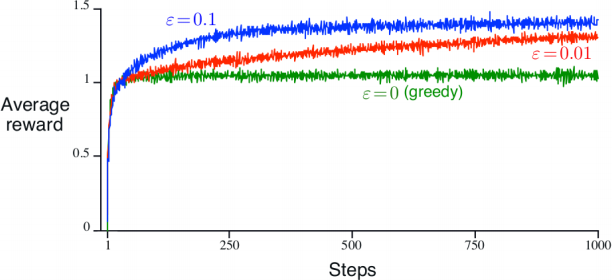
\includegraphics[width = 0.475 \textwidth]{1.3.1.png}
    }
    \subfloat
    {
        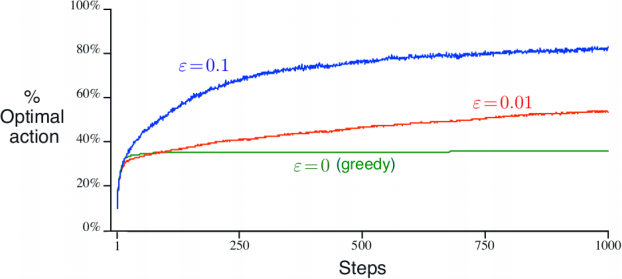
\includegraphics[width = 0.475 \textwidth]{1.3.2.png}
    }
    \hspace{0mm}
    \caption
    {
        Average performance of $\varepsilon$-greedy action-value methods on $10$-armed testbed.
        These data are averages over $2000$ runs with different bandit problems.
        All methods used sample averages as their action-value estimates.
    }
    \label{fig:1.3}
\end{figure}


\end{exercise}

\begin{solution}
In the long run the $\varepsilon = 0.01$-greedy action-value method will perform best. While the $\varepsilon = 0.1$ method does learn faster in the beginning, it will eventually be overtaken. This is because even if it has learned the best action to take, it will only take it in $91\%$ of cases, since it will still do exploration with a $10\%$ likelyhood. The $0.01$-method will, after it has learned the best action, take it in $99.1\%$ of the cases, since it does less exploration. The greedy method can not compete with them, it is likely to get stuck in a local optimum. The sweetspot seems to be to take $\varepsilon$ to be higher in the early steps, to find the optimal action as fast as possible and lower the parameter over time to guarantee that the best action, once learned, is performed more often.
\end{solution}
